\subsection{Observadores de estado (reconstruir variables que no se conocen)}

La retroalimentación de estado \( u = r - kx \) asume que todo el vector de estados es conocido \( x = [ x_{1}, x_{2}, \ldots, x_{n} ] \) y \( C=I \) para tener en la salida todas las variables de estado.
\[(1)
    \left\{
        \begin{array}{lll}
            \dot{x}(t) = Ax(t) + Bu(t) \\
            y(t) = Cx(t)
        \end{array}
    \right.
\]

\begin{figure}[ht]
    \centering
        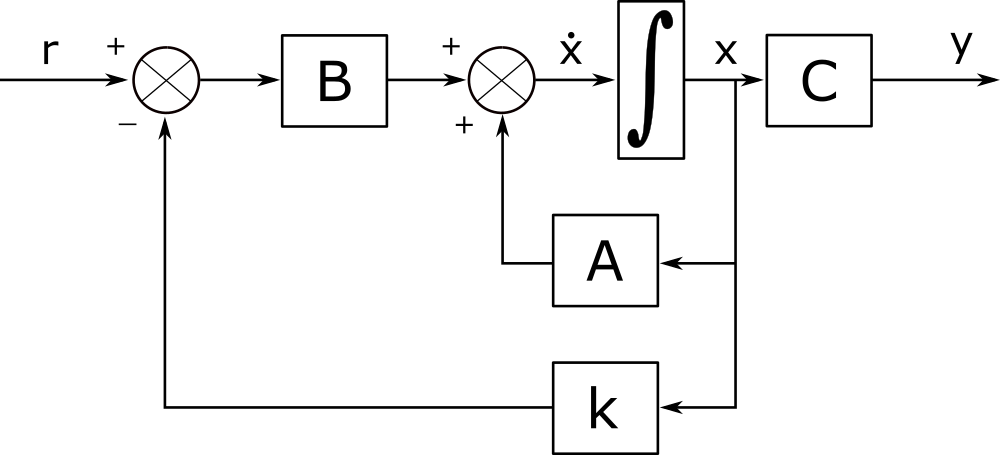
\includegraphics[scale=0.19]{Control de Sistemas Mecatronicos Figuras/08 Sistema Retroalimentado.png}
        \caption{Sistema retroalimentado}
\end{figure}

Sin embargo no siempre se tiene acceso a todas las variables de estado, debido a restricciones tecnológicas, de costos, etc,.

Los observadores de estado, se utilizan para aproximar el valor de las variables de estado desconocidas.

Sea \( x \) y \( \hat{x} \), donde \( \hat{x} \) es un valor aproximado del vector \( x \) obtenido mediante un observador de estado, entonces \( u = r - k\hat{x} \)
\begin{figure}[ht]
    \centering
        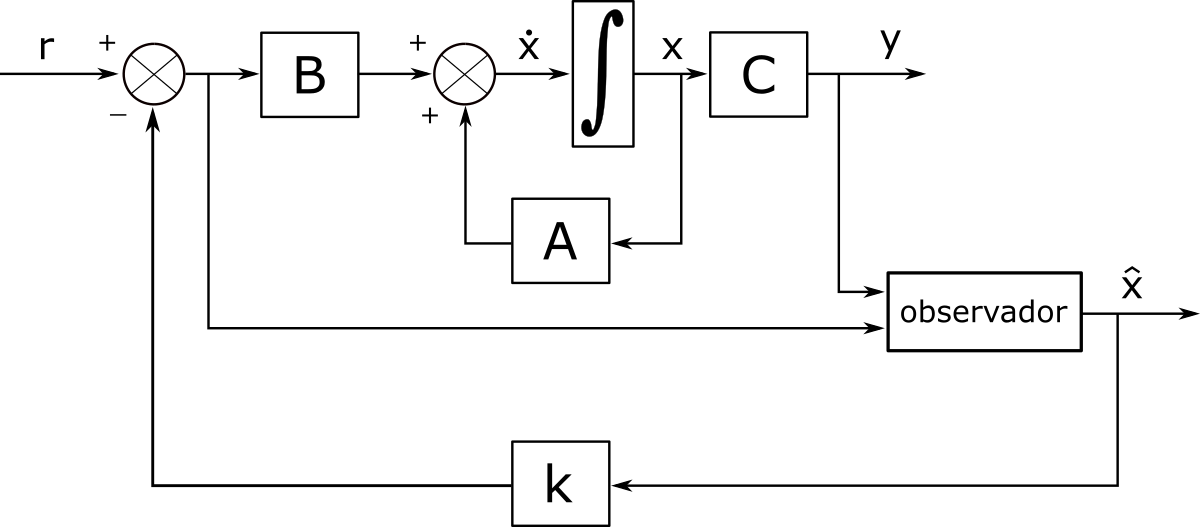
\includegraphics[scale=0.18]{Control de Sistemas Mecatronicos Figuras/09 Sistema Retroalimentado con Observador Propuesto.png}
        \caption{Sistema con observador}
\end{figure}

Se propone el observador de estado para (1)
\begin{figure}[ht]
    \centering
        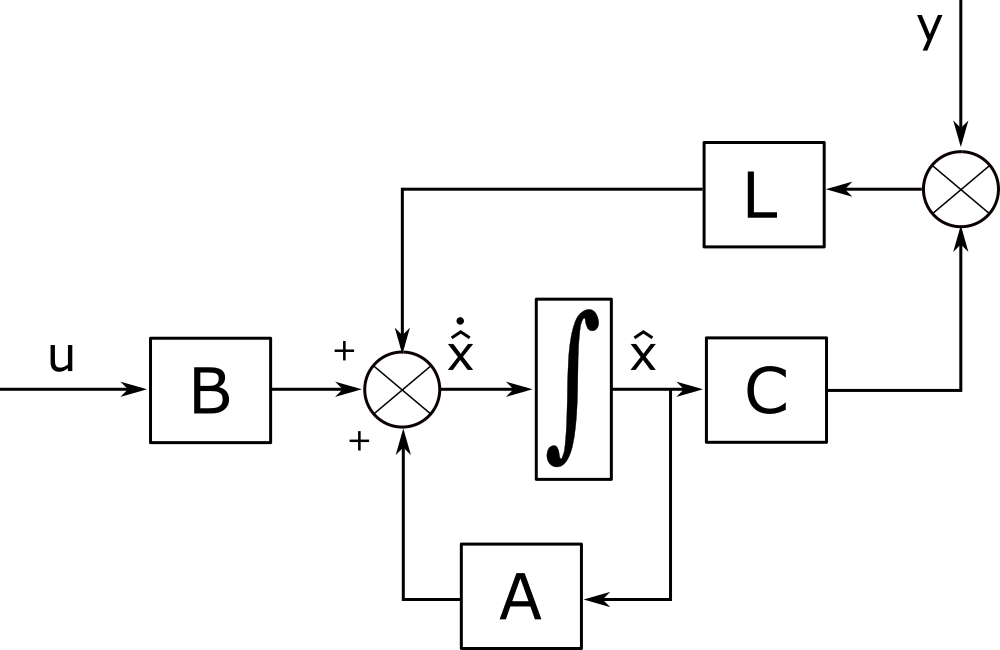
\includegraphics[scale=0.15]{Control de Sistemas Mecatronicos Figuras/10 Observador.png}
        \caption{Observador}
\end{figure}

\[
    \begin{split}
        \dot{\hat{x}} & = 
        \underbrace{A\hat{x} + Bu}_{
            \begin{matrix}
                \text{copia del} \\
                \text{del sistema}
            \end{matrix}}
            +
            \underbrace{L(y-C\hat{x})}_{
            \begin{matrix}
                \text{factor de} \\
                \text{corrección}
            \end{matrix}
            } \\
            & = A\hat{x} + Bu + Ly - LC\hat{x} \\
    \end{split}
\]

donde 
\[
    L = 
    \begin{bmatrix}
        L_{1} \\ L_{2} \\ \vdots \\ L_{n}
    \end{bmatrix}
\]

\begin{figure}[ht]
    \centering
        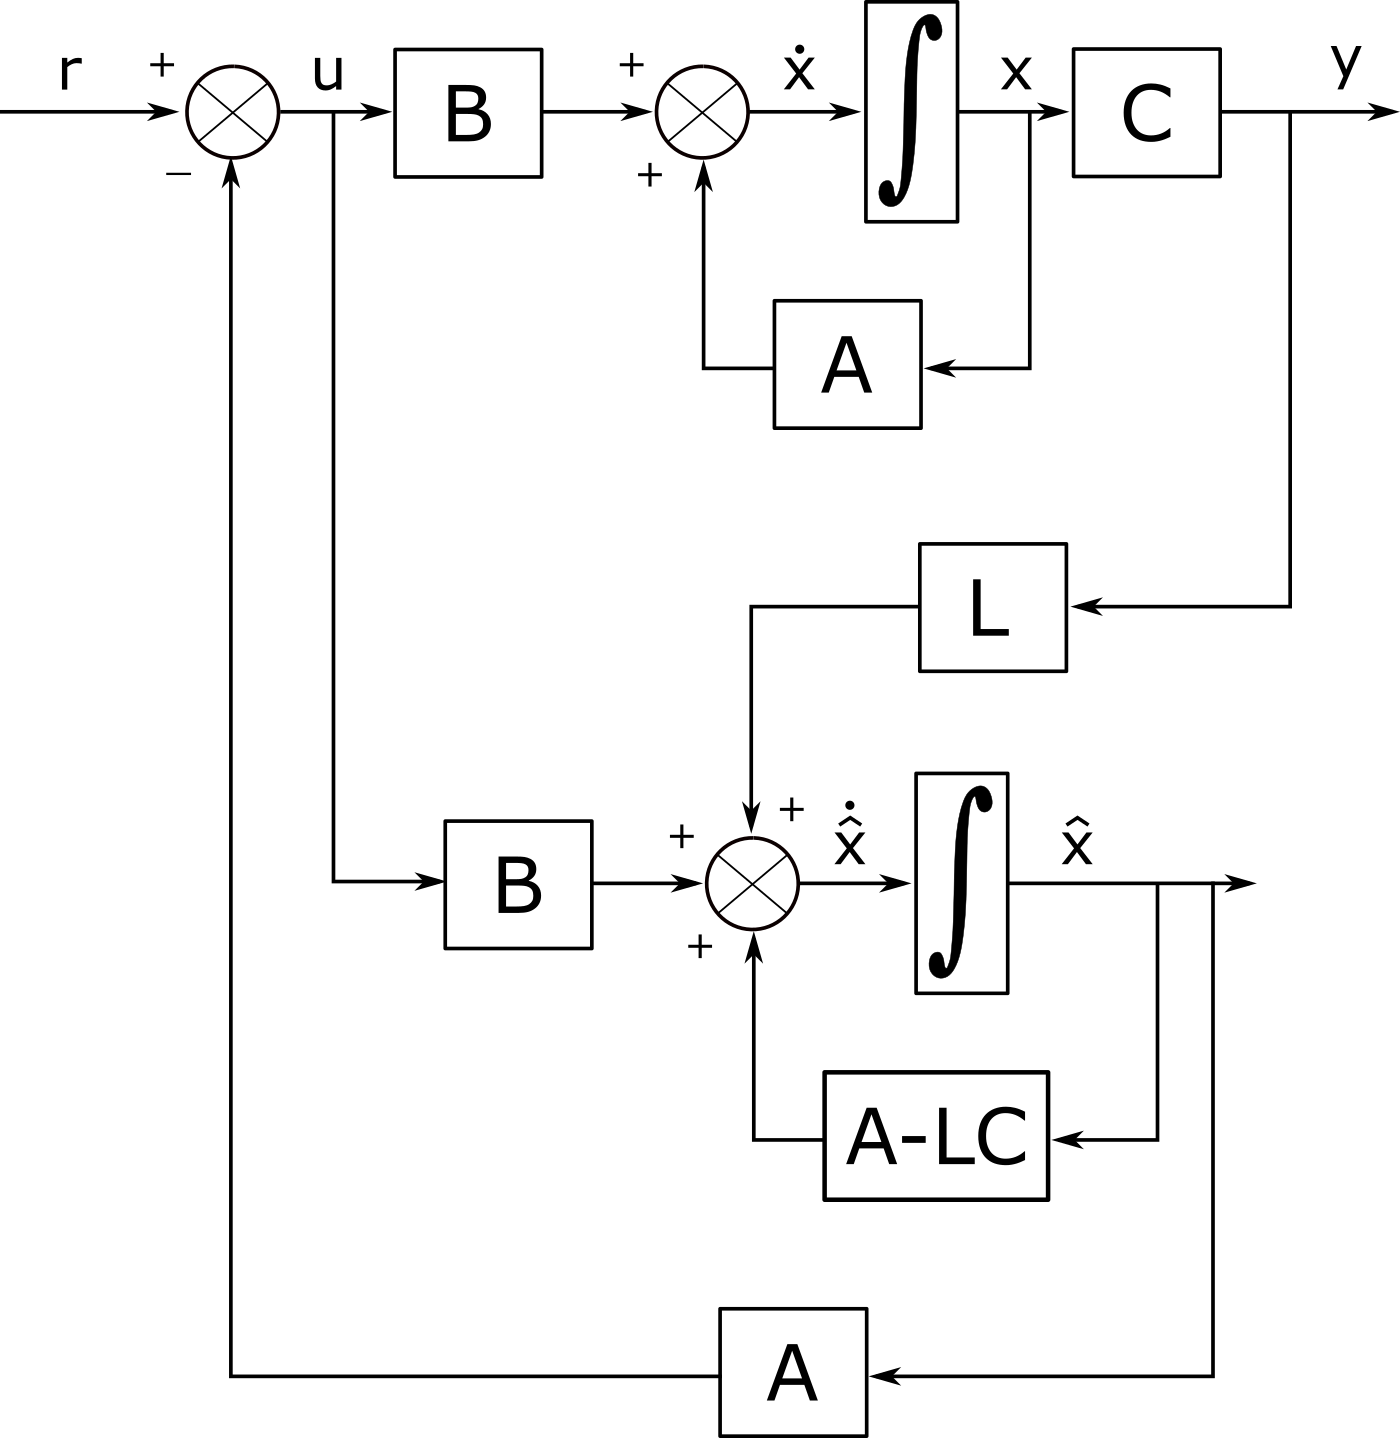
\includegraphics[scale=0.17]{Control de Sistemas Mecatronicos Figuras/11 Sistema con Observador Retroalimentado.png}
        \caption{Sistema con observador retroalimentado}
\end{figure}

\begin{figure}[h!]
    \centering
        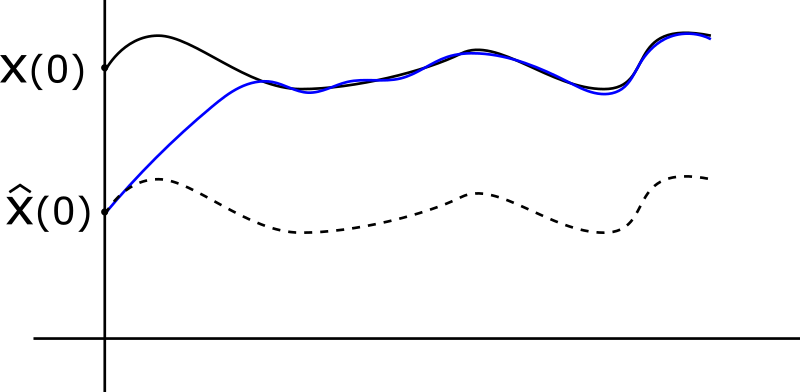
\includegraphics[scale=0.20]{Control de Sistemas Mecatronicos Figuras/12 Comparacion con Observador.png}
        \caption{Comparación con el observador de estado}
\end{figure}

Convergencia asintótica 
\[
    ||x - \hat{x}||\underset{t \to \inf}{\to} 0
\]
\[
    ||x-\hat{x}|| \le k_{0} e^{-\lambda t}
\]
\begin{figure}[h!]
    \centering
        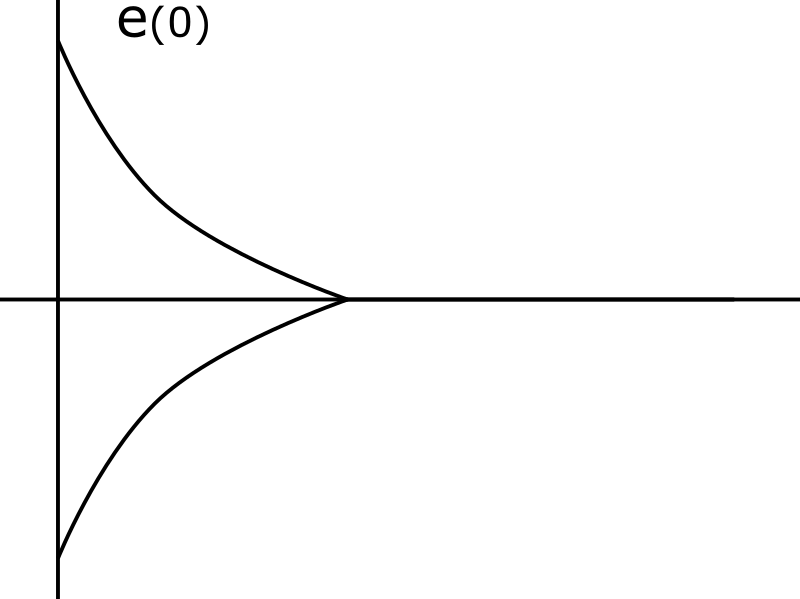
\includegraphics[scale=0.25]{Control de Sistemas Mecatronicos Figuras/13 Convergencia Asintotica.png}
        \caption{Comparación con el observador de estado}
\end{figure}

Se define el error de estimación 
\[
    (2) \;\; e(t) = x(t) -\hat{x}(t)
\]

Derivando (2) con respecto al tiempo
\[
    \begin{split}
        \dot{e}(t) & = \dot{x}(t) -\dot{\hat{x}}(t) \\
        & = Ax + Bu -A\hat{x} - Bu - L(y - C \hat{x}) \\
        & = Ax-A\hat{x}-L(Cx -C\hat{x})\\
        & = A
        \underbrace{ (x-\hat{x}) }_{ e(t) } 
        - LC
        \underbrace{ (x-\hat{x}) }_{ e(t) } \\
        & = Ae(t) - LCe(t) \\
        & = (A-LC)e(t) \;\; (3)
    \end{split}
\]

Para resolver la ecuación diferencial (3), se puede ver que \(f(t) = e(t)\) con condición inicial \(f(0) = e(0) \), y la derivada \( \dot{f(t)} = (A-LC)e(t) \). Así que se propone que \( f(t) =Q_{0}e^{Qt} \), por lo tanto se tiene que
\[
    f(0) = e(0) = Q_{0}e^{Q(0)}=Q_{0}e^{0} = Q_{o}I = Q_{0}
\]

La derivada de la función propuesta es 
\[
    \dot{f(t)} = Q_{0}Qe^{Qt}
\]

igualando funciones
\[
    \begin{split}
        Q_{0}Qe^{Qt} & = (A-LC)e(t) \\
        Q_{0}Qe^{Qt} & = (A-LC)Q_{0}e^{Qt} \\
        Q_{0}Qe^{Qt}(Q_{0}e^{Qt})^{-1} & = (A-LC)Q_{0}e^{Qt}(Q_{0}e^{Qt})^{-1}\\
        Q & = (A-LC) 
    \end{split}
\]

Sustituyendo \( Q \) y \( Q_{0} \) en la función propuesta 
\[
    f(t) = e(0)e^{(A-LC)t}
\]

El problema de diseño de observadores se resuelve como un problema de ubicación de polos, es decir, consiste en calcular \( L \) para asignar dinámica del observador de estado

\[
    \begin{split}
        P_{\text{obs}} & = det(sI-(A-LC)) \\
        & = (s-\mu_{1})(s-\mu_{2})\ldots(s-\mu_{n}) \\
        & = s^{n} + \tilde{a}_{1}s^{n-1} + \tilde{a}_{2}s^{n-2} + \ldots + \tilde{a}_{n} 
    \end{split}
\]